\begin{figure}
	\centering
	\pgfplotsset{every axis legend/.append style={
		at={(1.05,0.5)},
		anchor=west}}
	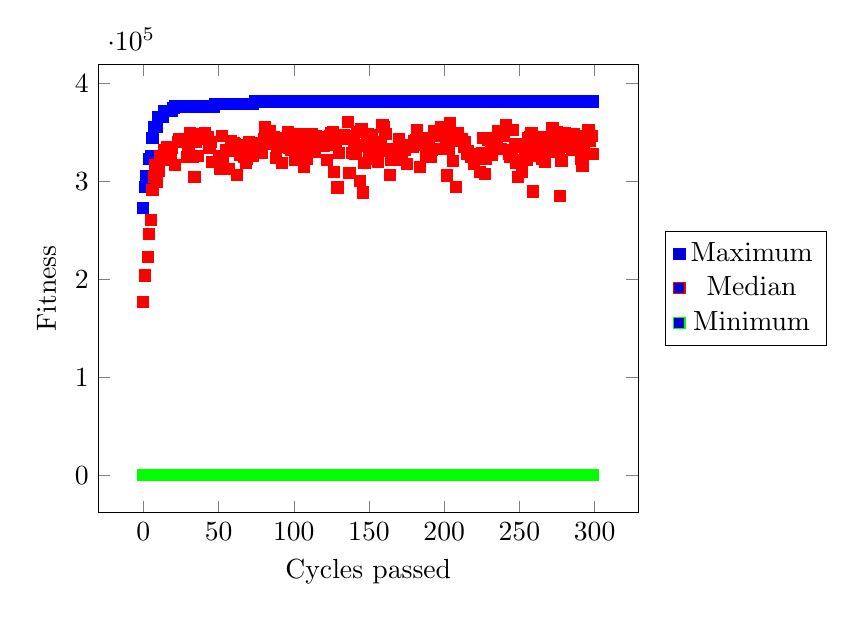
\begin{tikzpicture}
		\begin{axis}[
			xlabel=Cycles passed,
			ylabel=Fitness,
			scatter/classes={
				max={mark=square*,blue},
				med={mark=square*,red},
				min={mark=square*,green}
				}
            ]
            
\addplot+[scatter,only marks,scatter src=explicit symbolic]table[meta=label] {
x y label
0 272962 max
1 294172 max
2 304979 max
3 304979 max
4 322377 max
5 325684 max
6 344312 max
7 355718 max
8 355718 max
9 355718 max
10 365209 max
11 365209 max
12 365209 max
13 365209 max
14 372043 max
15 372043 max
16 372043 max
17 372043 max
18 372043 max
19 372043 max
20 375070 max
21 376222 max
22 376222 max
23 376269 max
24 376269 max
25 376269 max
26 376269 max
27 376269 max
28 376269 max
29 376269 max
30 376269 max
31 376269 max
32 376269 max
33 376269 max
34 376269 max
35 376269 max
36 376269 max
37 376269 max
38 376269 max
39 376269 max
40 376269 max
41 376269 max
42 376269 max
43 376269 max
44 376269 max
45 376269 max
46 376269 max
47 376269 max
48 379206 max
49 379206 max
50 379206 max
51 379206 max
52 379206 max
53 379206 max
54 379206 max
55 379206 max
56 379206 max
57 379206 max
58 379206 max
59 379206 max
60 379206 max
61 379206 max
62 379206 max
63 379206 max
64 379206 max
65 379206 max
66 379206 max
67 379206 max
68 379206 max
69 379206 max
70 379206 max
71 379206 max
72 379206 max
73 379206 max
74 381283 max
75 381283 max
76 381283 max
77 381283 max
78 381283 max
79 381283 max
80 381283 max
81 381283 max
82 381283 max
83 381283 max
84 381283 max
85 381283 max
86 381283 max
87 381283 max
88 381283 max
89 381283 max
90 381283 max
91 381283 max
92 381283 max
93 381283 max
94 381283 max
95 381283 max
96 381283 max
97 381283 max
98 381283 max
99 381283 max
100 381283 max
101 381283 max
102 381283 max
103 381283 max
104 381283 max
105 381283 max
106 381283 max
107 381283 max
108 381283 max
109 381283 max
110 381283 max
111 381283 max
112 381283 max
113 381283 max
114 381283 max
115 381283 max
116 381283 max
117 381283 max
118 381283 max
119 381283 max
120 381283 max
121 381283 max
122 381283 max
123 381283 max
124 381283 max
125 381283 max
126 381283 max
127 381283 max
128 381283 max
129 381283 max
130 381283 max
131 381283 max
132 381283 max
133 381283 max
134 381283 max
135 381283 max
136 381283 max
137 381283 max
138 381283 max
139 381283 max
140 381283 max
141 381283 max
142 381283 max
143 381283 max
144 381283 max
145 381283 max
146 381283 max
147 381283 max
148 381283 max
149 381283 max
150 381283 max
151 381283 max
152 381283 max
153 381283 max
154 381283 max
155 381283 max
156 381283 max
157 381283 max
158 381283 max
159 381283 max
160 381283 max
161 381283 max
162 381283 max
163 381283 max
164 381283 max
165 381283 max
166 381283 max
167 381283 max
168 381283 max
169 381283 max
170 381283 max
171 381283 max
172 381283 max
173 381283 max
174 381283 max
175 381283 max
176 381283 max
177 381283 max
178 381283 max
179 381283 max
180 381283 max
181 381283 max
182 381283 max
183 381283 max
184 381283 max
185 381283 max
186 381283 max
187 381283 max
188 381283 max
189 381283 max
190 381283 max
191 381283 max
192 381283 max
193 381283 max
194 381283 max
195 381283 max
196 381283 max
197 381283 max
198 381283 max
199 381283 max
200 381283 max
201 381283 max
202 381283 max
203 381283 max
204 381283 max
205 381283 max
206 381283 max
207 381283 max
208 381283 max
209 381283 max
210 381283 max
211 381283 max
212 381283 max
213 381283 max
214 381283 max
215 381283 max
216 381283 max
217 381283 max
218 381283 max
219 381283 max
220 381283 max
221 381283 max
222 381283 max
223 381283 max
224 381283 max
225 381283 max
226 381283 max
227 381283 max
228 381283 max
229 381283 max
230 381283 max
231 381283 max
232 381283 max
233 381283 max
234 381283 max
235 381283 max
236 381283 max
237 381283 max
238 381283 max
239 381283 max
240 381283 max
241 381283 max
242 381283 max
243 381283 max
244 381283 max
245 381283 max
246 381283 max
247 381283 max
248 381283 max
249 381283 max
250 381283 max
251 381283 max
252 381283 max
253 381283 max
254 381283 max
255 381283 max
256 381283 max
257 381283 max
258 381283 max
259 381283 max
260 381283 max
261 381283 max
262 381283 max
263 381283 max
264 381283 max
265 381283 max
266 381283 max
267 381283 max
268 381283 max
269 381283 max
270 381283 max
271 381283 max
272 381283 max
273 381283 max
274 381283 max
275 381283 max
276 381283 max
277 381283 max
278 381283 max
279 381283 max
280 381283 max
281 381283 max
282 381283 max
283 381283 max
284 381283 max
285 381283 max
286 381283 max
287 381283 max
288 381283 max
289 381283 max
290 381283 max
291 381283 max
292 381283 max
293 381283 max
294 381283 max
295 381283 max
296 381283 max
297 381283 max
298 381283 max
299 381283 max
};
\addplot+[scatter,only marks,scatter src=explicit symbolic]table[meta=label] {
x y label
0 177071 med
1 203689 med
2 0 med
3 222387 med
4 246048 med
5 260727 med
6 291266 med
7 304652 med
8 316684 med
9 298856 med
10 310895 med
11 325529 med
12 325482 med
13 321731 med
14 331839 med
15 328313 med
16 334896 med
17 329355 med
18 323019 med
19 333846 med
20 0 med
21 316644 med
22 0 med
23 339992 med
24 342835 med
25 342805 med
26 342835 med
27 340190 med
28 340704 med
29 324668 med
30 337383 med
31 349165 med
32 344293 med
33 324633 med
34 304581 med
35 340190 med
36 325480 med
37 0 med
38 0 med
39 348192 med
40 344691 med
41 349100 med
42 343403 med
43 345092 med
44 334234 med
45 340273 med
46 319303 med
47 0 med
48 0 med
49 0 med
50 325604 med
51 312062 med
52 346244 med
53 319819 med
54 0 med
55 331326 med
56 331272 med
57 312549 med
58 340870 med
59 333786 med
60 339221 med
61 337450 med
62 306591 med
63 0 med
64 326695 med
65 336640 med
66 326920 med
67 324321 med
68 318680 med
69 322584 med
70 340262 med
71 330146 med
72 335143 med
73 325497 med
74 338768 med
75 333000 med
76 334234 med
77 335436 med
78 334852 med
79 328772 med
80 343356 med
81 355122 med
82 347683 med
83 349834 med
84 350694 med
85 337716 med
86 337774 med
87 344868 med
88 323601 med
89 335175 med
90 337038 med
91 0 med
92 318810 med
93 0 med
94 344138 med
95 335875 med
96 350265 med
97 334234 med
98 332342 med
99 332587 med
100 342070 med
101 321539 med
102 335462 med
103 340572 med
104 348307 med
105 336521 med
106 332861 med
107 314439 med
108 0 med
109 322328 med
110 337864 med
111 336001 med
112 348476 med
113 335931 med
114 330240 med
115 345633 med
116 342224 med
117 345069 med
118 340572 med
119 0 med
120 336436 med
121 341654 med
122 321849 med
123 337716 med
124 345765 med
125 349532 med
126 349834 med
127 309110 med
128 336638 med
129 293592 med
130 328578 med
131 345598 med
132 344135 med
133 346690 med
134 342983 med
135 345939 med
136 360185 med
137 308738 med
138 0 med
139 328471 med
140 337439 med
141 328112 med
142 350516 med
143 337203 med
144 300592 med
145 353476 med
146 288533 med
147 318993 med
148 335942 med
149 348380 med
150 326902 med
151 346917 med
152 345074 med
153 322385 med
154 335366 med
155 0 med
156 319546 med
157 331532 med
158 339869 med
159 357042 med
160 355613 med
161 348380 med
162 330740 med
163 0 med
164 306252 med
165 321888 med
166 332861 med
167 0 med
168 332587 med
169 332732 med
170 343193 med
171 321603 med
172 324959 med
173 336393 med
174 331503 med
175 317276 med
176 0 med
177 0 med
178 0 med
179 334561 med
180 340572 med
181 341789 med
182 352037 med
183 338783 med
184 314294 med
185 337152 med
186 337716 med
187 343656 med
188 324421 med
189 333817 med
190 341789 med
191 324959 med
192 331433 med
193 351258 med
194 332448 med
195 332448 med
196 345759 med
197 350704 med
198 355603 med
199 347163 med
200 346643 med
201 341535 med
202 305861 med
203 333351 med
204 358979 med
205 341789 med
206 320440 med
207 345759 med
208 294483 med
209 349178 med
210 340906 med
211 343403 med
212 343403 med
213 335476 med
214 340084 med
215 327524 med
216 330240 med
217 327598 med
218 324959 med
219 0 med
220 318110 med
221 0 med
222 0 med
223 0 med
224 309524 med
225 328231 med
226 344326 med
227 307319 med
228 322800 med
229 342224 med
230 344326 med
231 329465 med
232 327042 med
233 341061 med
234 336701 med
235 336638 med
236 350694 med
237 350056 med
238 333101 med
239 346127 med
240 350056 med
241 356891 med
242 0 med
243 328157 med
244 325194 med
245 331378 med
246 351911 med
247 337800 med
248 318590 med
249 304471 med
250 337976 med
251 321640 med
252 309786 med
253 335116 med
254 331532 med
255 322218 med
256 344483 med
257 345246 med
258 349018 med
259 289567 med
260 331494 med
261 325699 med
262 334798 med
263 340066 med
264 345074 med
265 323150 med
266 327396 med
267 319694 med
268 334694 med
269 340300 med
270 331340 med
271 341109 med
272 353767 med
273 330079 med
274 346484 med
275 350056 med
276 332006 med
277 285002 med
278 321186 med
279 334678 med
280 349067 med
281 336880 med
282 345074 med
283 337152 med
284 334537 med
285 331532 med
286 347838 med
287 341789 med
288 340859 med
289 345759 med
290 338246 med
291 322795 med
292 315702 med
293 330977 med
294 343018 med
295 345882 med
296 352222 med
297 340906 med
298 345765 med
299 327560 med
};
\addplot+[scatter,only marks,scatter src=explicit symbolic]table[meta=label] {
x y label
0 0 min
1 0 min
2 0 min
3 0 min
4 0 min
5 0 min
6 0 min
7 0 min
8 0 min
9 0 min
10 0 min
11 0 min
12 0 min
13 0 min
14 0 min
15 0 min
16 0 min
17 0 min
18 0 min
19 0 min
20 0 min
21 0 min
22 0 min
23 0 min
24 0 min
25 0 min
26 0 min
27 0 min
28 0 min
29 0 min
30 0 min
31 0 min
32 0 min
33 0 min
34 0 min
35 0 min
36 0 min
37 0 min
38 0 min
39 0 min
40 0 min
41 0 min
42 0 min
43 0 min
44 0 min
45 0 min
46 0 min
47 0 min
48 0 min
49 0 min
50 0 min
51 0 min
52 0 min
53 0 min
54 0 min
55 0 min
56 0 min
57 0 min
58 0 min
59 0 min
60 0 min
61 0 min
62 0 min
63 0 min
64 0 min
65 0 min
66 0 min
67 0 min
68 0 min
69 0 min
70 0 min
71 0 min
72 0 min
73 0 min
74 0 min
75 0 min
76 0 min
77 0 min
78 0 min
79 0 min
80 0 min
81 0 min
82 0 min
83 0 min
84 0 min
85 0 min
86 0 min
87 0 min
88 0 min
89 0 min
90 0 min
91 0 min
92 0 min
93 0 min
94 0 min
95 0 min
96 0 min
97 0 min
98 0 min
99 0 min
100 0 min
101 0 min
102 0 min
103 0 min
104 0 min
105 0 min
106 0 min
107 0 min
108 0 min
109 0 min
110 0 min
111 0 min
112 0 min
113 0 min
114 0 min
115 0 min
116 0 min
117 0 min
118 0 min
119 0 min
120 0 min
121 0 min
122 0 min
123 0 min
124 0 min
125 0 min
126 0 min
127 0 min
128 0 min
129 0 min
130 0 min
131 0 min
132 0 min
133 0 min
134 0 min
135 0 min
136 0 min
137 0 min
138 0 min
139 0 min
140 0 min
141 0 min
142 0 min
143 0 min
144 0 min
145 0 min
146 0 min
147 0 min
148 0 min
149 0 min
150 0 min
151 0 min
152 0 min
153 0 min
154 0 min
155 0 min
156 0 min
157 0 min
158 0 min
159 0 min
160 0 min
161 0 min
162 0 min
163 0 min
164 0 min
165 0 min
166 0 min
167 0 min
168 0 min
169 0 min
170 0 min
171 0 min
172 0 min
173 0 min
174 0 min
175 0 min
176 0 min
177 0 min
178 0 min
179 0 min
180 0 min
181 0 min
182 0 min
183 0 min
184 0 min
185 0 min
186 0 min
187 0 min
188 0 min
189 0 min
190 0 min
191 0 min
192 0 min
193 0 min
194 0 min
195 0 min
196 0 min
197 0 min
198 0 min
199 0 min
200 0 min
201 0 min
202 0 min
203 0 min
204 0 min
205 0 min
206 0 min
207 0 min
208 0 min
209 0 min
210 0 min
211 0 min
212 0 min
213 0 min
214 0 min
215 0 min
216 0 min
217 0 min
218 0 min
219 0 min
220 0 min
221 0 min
222 0 min
223 0 min
224 0 min
225 0 min
226 0 min
227 0 min
228 0 min
229 0 min
230 0 min
231 0 min
232 0 min
233 0 min
234 0 min
235 0 min
236 0 min
237 0 min
238 0 min
239 0 min
240 0 min
241 0 min
242 0 min
243 0 min
244 0 min
245 0 min
246 0 min
247 0 min
248 0 min
249 0 min
250 0 min
251 0 min
252 0 min
253 0 min
254 0 min
255 0 min
256 0 min
257 0 min
258 0 min
259 0 min
260 0 min
261 0 min
262 0 min
263 0 min
264 0 min
265 0 min
266 0 min
267 0 min
268 0 min
269 0 min
270 0 min
271 0 min
272 0 min
273 0 min
274 0 min
275 0 min
276 0 min
277 0 min
278 0 min
279 0 min
280 0 min
281 0 min
282 0 min
283 0 min
284 0 min
285 0 min
286 0 min
287 0 min
288 0 min
289 0 min
290 0 min
291 0 min
292 0 min
293 0 min
294 0 min
295 0 min
296 0 min
297 0 min
298 0 min
299 0 min
};

			\addlegendentry{Maximum}
			\addlegendentry{Median}
			\addlegendentry{Minimum}
		\end{axis}
	\end{tikzpicture}
	\caption{Detail of genetic algorithm on balanced data with 30 elements in set and mutation chance of 1/1024}
\label{plot:genProfile30-mutation1024}
\end{figure}
